\documentclass[11pt,letter, swedish, english
]{article}
\pdfoutput=1

\usepackage{../custom_as}

\usepackage{listings} 
\usepackage[framed,numbered,autolinebreaks,useliterate]{../mcode}
\lstloadlanguages{matlab} 
\lstset{language=matlab} 

\usepackage[makeroom]{cancel}
\graphicspath{{figures/}}


\swapcommands{\Omega}{\varOmega}

%%Drar in tabell och figurtexter
\usepackage[margin=10 pt]{caption}
%%För att lägga in 'att göra'-noteringar i texten
\usepackage{todonotes} %\todo{...}

%%För att själv bestämma marginalerna. 
\usepackage[
%            top    = 2.5cm,
%            bottom = 3cm,
%            left   = 3cm, right  = 3cm
]{geometry}

%%För att ändra hur rubrikerna ska formateras


%\renewcommand{\thefootnote}{\fnsymbol{footnote}}

\renewcommand{\thesubsection}{\arabic{section} (\alph{subsection})}
\renewcommand{\thesubsubsection}{\arabic{section} (\alph{subsection},\,\roman{subsubsection})}


\begin{document}




%%%%%%%%%%%%%%%%% vvv Inbyggd titelsida vvv %%%%%%%%%%%%%%%%%

\title{Numerical solutions to PDE's -- AMATH\,741 \\
Assignment 1}
\author{Andréas Sundström}
\date{\today}

\maketitle

%%%%%%%%%%%%%%%%% ^^^ Inbyggd titelsida ^^^ %%%%%%%%%%%%%%%%%

\section{Advection-diffusion equation}

Here we will consider the equation
\begin{equation}\label{eq:1_start}
u_t+au_x=\sigma u_{xx}\qcomma
a>0\qcomma \sigma>0
\end{equation}
on some domain.
The solutions are assumed to be of the form
\begin{equation}\label{eq:1_sol1}
u(x, t)=\sum_k \hat{u}(k, t)\ee^{\ii kx}.
\end{equation}
(The exact specification of $k$ in the sum is not given here. That is
because the values of $k$ depends on the IC or BC.)

\subsection{Finding a solution}
To find the form of each term in \eqref{eq:1_sol1}, we can omit the
sum in \eqref{eq:1_sol1}, since the governing PDE is linear. We get
\begin{equation}\label{eq:1_disp}
\hat{u}_t + \ii ka\, \hat{u}
=-\sigma k^2\hat{u},
\end{equation}
where we've also canceled the factor $ee^{\ii kx}$ appearing in all of
the terms in the dispersion relation \eqref{eq:1_disp}. We see now
that \eqref{eq:1_disp} is a DE in $t$ with the solution
\begin{equation}
\hat{u}(k, t)= c(k)\, \ee^{-(\ii ka+\sigma k^2)t},
\end{equation}
where $c(k)$ is some function of $k$ (that depends on the I.C.).
The solution to \eqref{eq:1_start} thus becomes
\begin{equation}\label{eq:1_sol2}
u(x, t) = \sum_k c(k)\, \ee^{\ii k(x-at)}\ee^{-\sigma k^2t}.
\end{equation}

The initial conditions come into play on determining $c(k)$. Let's say
that
\begin{equation}
u(x, 0)=\varphi(x)
\end{equation}
on the domain of the problem. Then, setting $t=0$ in
\eqref{eq:1_sol2}, we get
\begin{equation}\label{eq:1_F-series}
\sum_k c(k)\, \ee^{\ii kx}=\varphi(x)
\end{equation}
This is a Fourier series expansion of $\varphi$; for this to work we
need $\varphi$ to be piecewise continuous and either of these two
cases must to be satisfied
\begin{enumerate}[label=\Roman*.]
\item the domain of the problem is bounded with length $P$,
\item or $\varphi$ is periodic with period $P$,
\end{enumerate}
and also that $\varphi\in\mathcal{L}^2[x_0, x_0+P]$.
The allowed frequencies will be $k=n/P$, $n\in\Z$.
And the coefficients are the regular Fourier coefficients
\begin{equation}
c(k)=\frac{1}{P}\int_{x_0}^{x_0+P} \varphi(x)\ee^{-\ii kx}\id{x}.
\end{equation}

An example of a possible IC of the first kind would be 
\begin{equation}
\varphi_\mathrm{I}(x)=1-|x|
\end{equation}
on the finite domain $x\in[-1, 1]$. An example of the second kind of
IC could be
\begin{equation}
\varphi_\mathrm{II}(x)=\cos(x)+\cos(2x)
\end{equation}
on $x\in\R$.


\subsection{Periodic boundary conditions}
\begin{figure}\centering
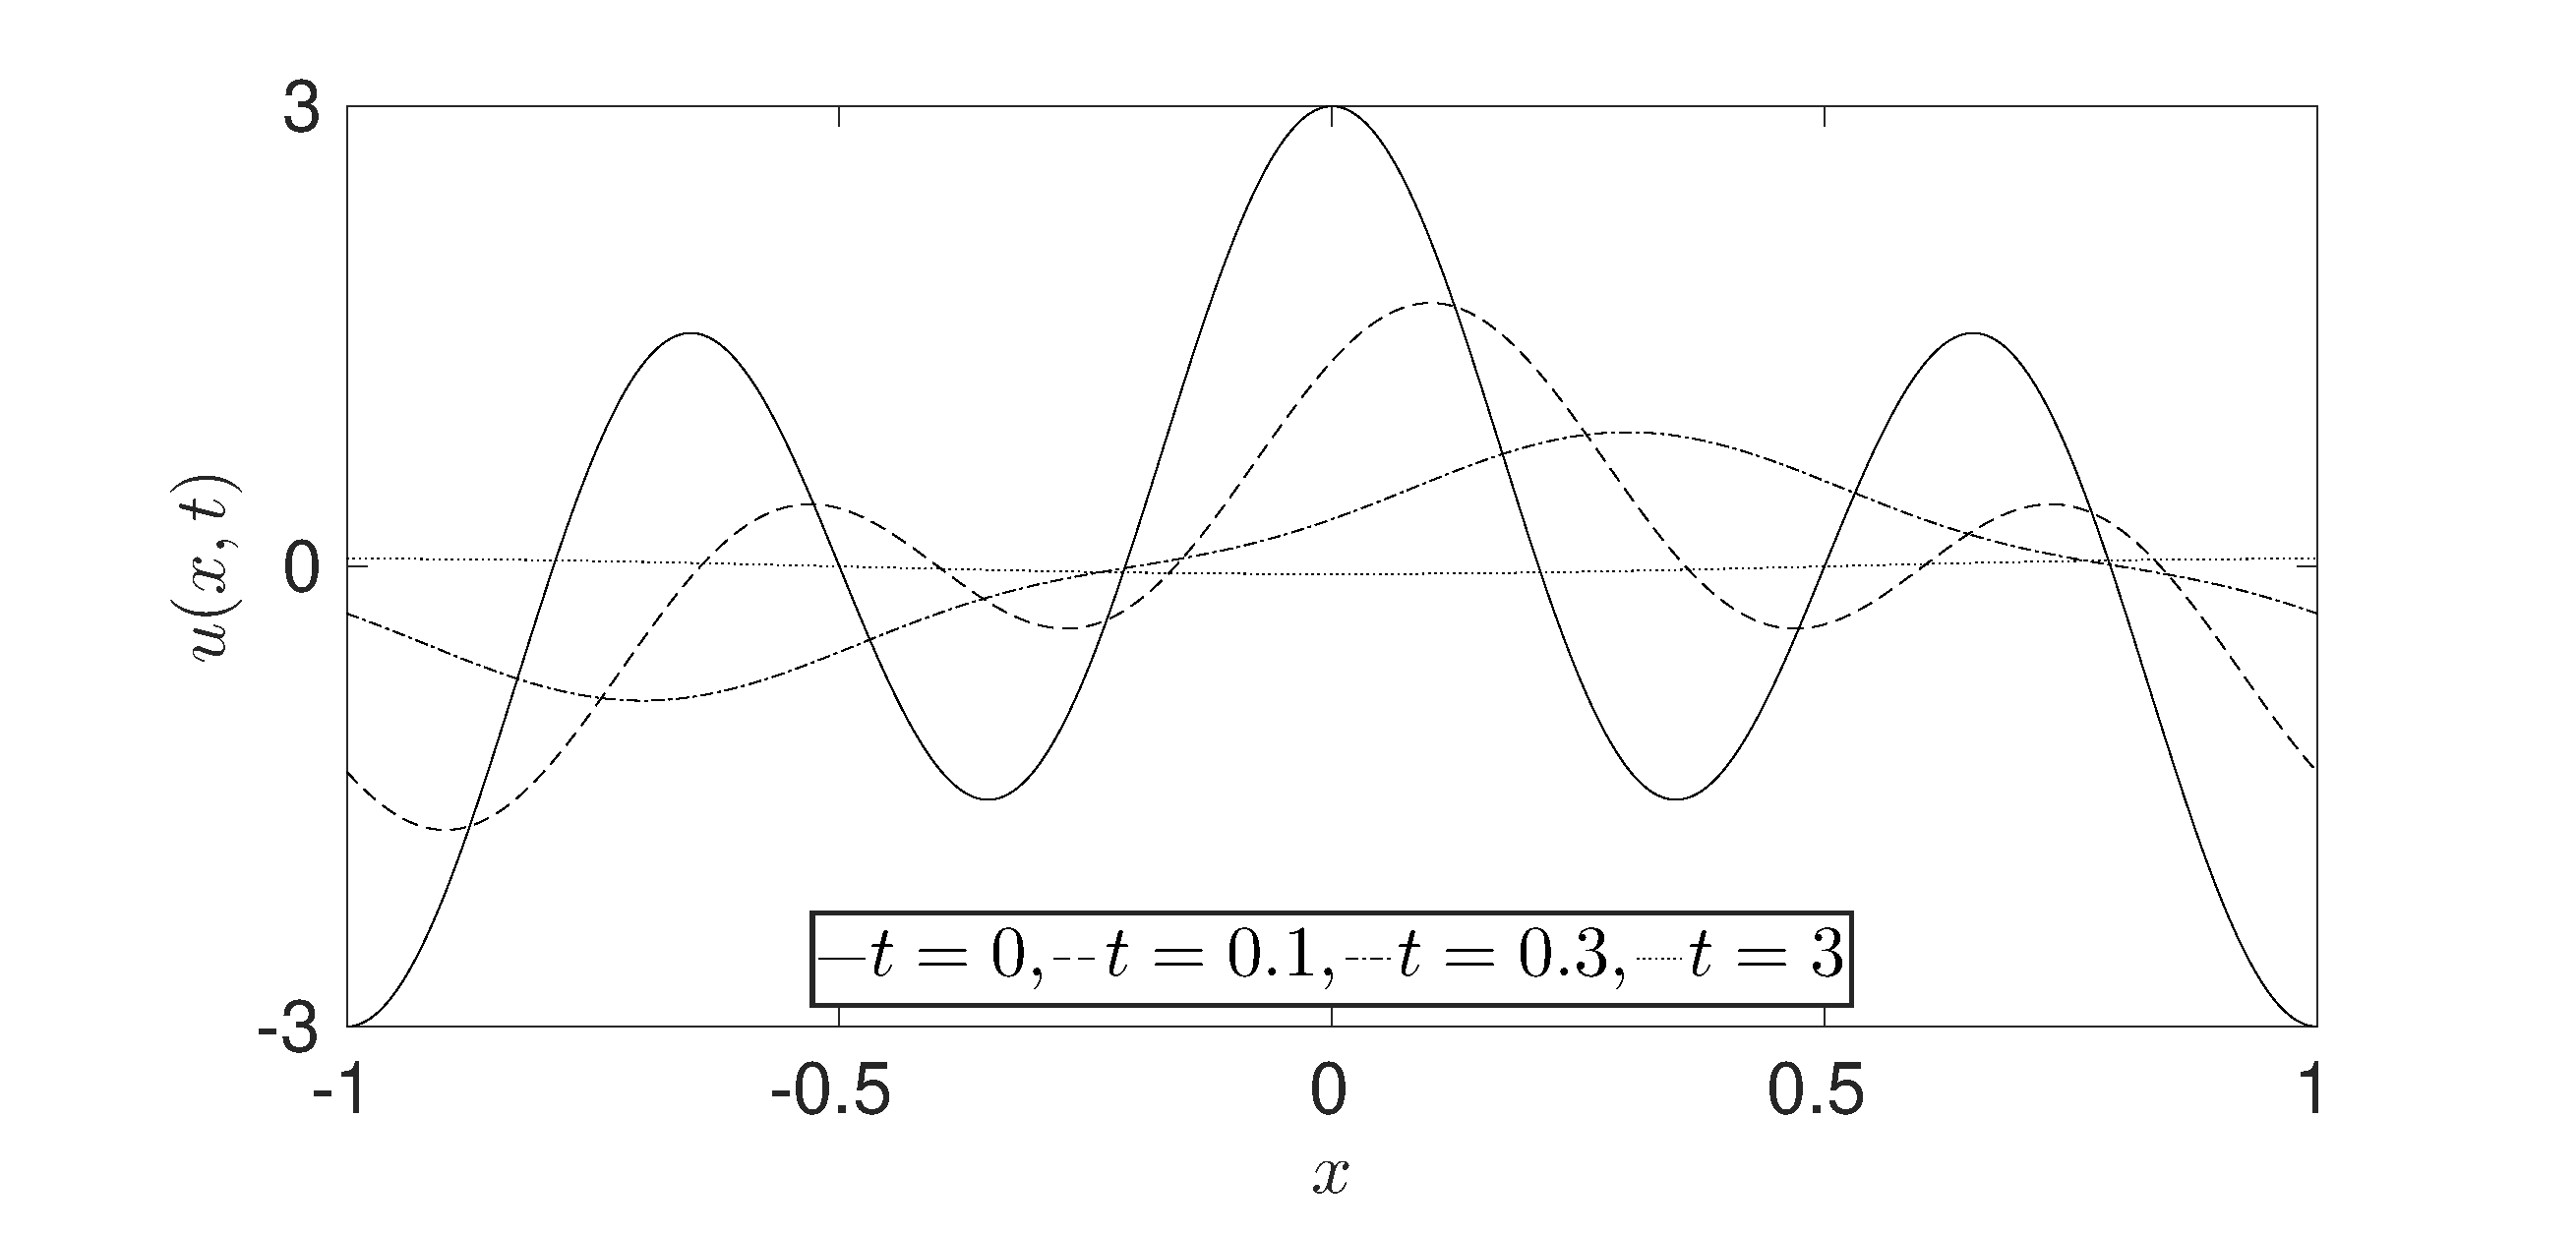
\includegraphics[width=.8\textwidth]{1_time_evolution.eps}
\caption{The time evolution of a solution to \eqref{eq:1_start} with
  periodic BC. The parameter values and IC are: $\sigma=a=1$ and 
  $\varphi(x)=\cos(\pi x)+2\cos(3\pi x)$. We see how, at $t=0.2$, the
  general form of the function is shifted to the right and not
  distorted very much; but at $t=0.3$ we also see that the high
  frequency component have been attenuated more; at $t=3$ almost all
  of the fluctuations are gone.}
\label{fig:1}
\end{figure}

Periodic boundary conditions are equivalent to changing from case I to
case II. 

What will happen is that each frequency will be attenuated according
to $\ee^{-\sigma k^2t}$, and then Fourier analysis tells us that the
(space domain) solution will be shifted\footnotemark{} by $at$ (to
the right for $t>0$). 

\footnotetext{See part (c) of this problem for more details.}

An example of this behavior is shown in \figref{fig:1}.

\subsection{Relating this solution to the solutions of the original PDE's}
As said before the factor $\ee^{-\ii kat}$, resulting from the term
$au_x$ in \eqref{eq:1_start}, translates the solution in the positive
direction of the $x$-axis with time. To see this we have to go back to
the Fourier series \eqref{eq:1_F-series}; if we multiply the LHS by
$\ee^{-\ii kat}$ and change variables to $y=x-at$, we see that
\begin{equation}
\sum_k c(k)\, \ee^{\ii k(x-at)}=\sum_k c(k)\, \ee^{\ii ky}
\stackrel{\eqref{eq:1_F-series}}{=}\varphi(y)=\varphi(x-at).
\end{equation}
This is the behavior expected if $\sigma=0$, i.e. when we only have
the advection equation. This is also the exact behavior of solutions
to the advection equations. 

In the other case, where $a=0$, we see that 
\begin{equation}
u(x, t) = \sum_k c(k)\, \ee^{\ii kx}\ee^{-\sigma k^2t}.
\end{equation}
Where basically each frequency component get attenuated based on the
frequency. This is the exact behavior expected from a solution to the
pure heat equation. 

Together we get a mix of both. The whole solution gets shifted to the
right (due to the advection part), while each frequency component at
the same time gets attenuated (due to the heat equation part). 




\section{Higher order approximations of derivatives}
\newcommand{\Dx}{\ensuremath{\Delta{x}}}
We want to find approximations to derivatives to some reasonably
smooth function $u$, using the functional values from points away from
the point of interest. In other words, we are looking for $C_i$ such
that\footnotemark{}
\begin{equation}\label{eq:2_start}
u_{dx}=\frac{d!}{\Dx^d} \sum_i C_i u(x+i\Dx) \quad+\order{\Dx^E},
\end{equation}
where
\begin{equation}
u_{dx}:=\pdv[d]{u}{x}
\end{equation}
is the definition of the notation, $E$ is some order of the truncation
error and the sum is some given set of $i$'s.
\footnotetext{The $t$ dependence have not been written out explicitly
  since this problem only concerns derivatives of one kind.}


We can begin by Taylor expanding $u(x+i\Dx)$:
\begin{equation}\label{eq:2_Taylor0}
u(x+i\Dx) = \sum_{n=0}^{d+E-1}
\frac{i^n\Dx^n}{n!} u_{nx}(x)
\quad+\order{\Dx^{d+E}}
\end{equation}
The expansion is done up to order $d+E-1$ because that's all we need
given the error in \eqref{eq:2_start}. Now substitute
\eqref{eq:2_Taylor0} into \eqref{eq:2_start}: 
\begin{equation}
u_{dx}=\frac{d!}{\Dx^d} \sum_{n=0}^{d+E-1}
\frac{\Dx^n}{n!} u_{nx}(x) \sum_i i^nC_i 
\quad+\order{\Dx^E}.
\end{equation}
Note that the order of the sums have been switched; this is okay since
we're only dealing with finite sums. 

Now if we disregard the error term at the end, we see that for the RHS
to be equal to the LHS $C_i$ have to be such that\footnotemark{}
\begin{equation}
\sum_i i^nC_i=
\begin{cases}
1\qcomma&n=d,\\
0,& n\neq d.
\end{cases}
\end{equation}
This is a linear system of equations 
\begin{equation}
\mathsf{A}\vb*{C}=[0, \ldots, 0, 1, 0, \ldots, 0]^\mathsfrm{T}
\end{equation}
with $I=$ ``the number of different
$i$'s'' unknowns, so we need $I$ equations; that is $I=d+E$. Basically
the number of $i$'s is determined by the order of the derivative and
how much error you want. 
Once the system of equations is solved, we get our approximation to
the derivative by plugging the $C_i$'s back into \eqref{eq:2_start}.

\footnotetext{As always with Taylor expansions, we assume the convention
that $``0^0"=1$.}

\subsection{Second and third derivative}
Here we will be using $u_j$, $u_{j\pm1}$ and $u_{j\pm2}$ to
approximate $(u_{xx})_j^n$ and $(u_{xxx})_j^n$. We see that we have
$I=5$ different values of $i\in\{-2, -1, 0, 1, 2\}$, so we have a
$5\times5$ system of equations with the matrix
\begin{equation}
\mathsf{A}=
\begin{bmatrix*}[r]
1&1&1&1&1\\
-2&-1&0&1&2\\
4&1&0&1&4\\
-8&-1&0&1&8\\
16&1&0&1&16
\end{bmatrix*}.
\end{equation}

For the second derivative we have
\begin{equation}
\mathsf{A}\vb*{C}=[0, 0, 1, 0, 0]^\mathsfrm{T},
\end{equation}
which has the solution
\begin{equation}
\vb*{C}=\frac{1}{24}[-1, 16, -30, 16, -1]^\mathsfrm{T}.
\end{equation}
When plugged back into \eqref{eq:2_start}, we get
\begin{equation}
(u_{xx})_j^n=\frac{-u_{j+2}^n+16u_{j+1}^n-30u_{j}^n+16u_{j-1}^n-u_{j-2}^n}{12\Dx^2}
+\order{\Dx^4}.
\end{equation}
Note that according to the prescription $I=d+E$ we should have gotten
$\order{\Dx^3}$ as the error, but due to the symmetry in the Taylor
expansion the $\Dx^3$ term vanishes. 

For the third derivative we get
\begin{equation}
\mathsf{A}\vb*{C}=[0, 0, 0, 1, 0]^\mathsfrm{T},
\end{equation}
which has the solution
\begin{equation}
\vb*{C}=\frac{1}{12} [-1, 2, 0, -2, 1]^\mathsfrm{T}.
\end{equation}
When plugged back into \eqref{eq:2_start}, we get
\begin{equation}
(u_{xxx})_j^n=\frac{-u_{j+2}^n+2u_{j+1}^n-2u_{j-1}^n+u_{j-2}^n}{2\Dx^3}
+\order{\Dx^2}.
\end{equation}

\subsection{Fourth forward derivative}
The method presented in the beginning of this problem is general. All
we need to do is to pick what error we want, and then we know how many
steps we need. The only thing to keep in mind is that we're looking
for a \emph{forward} derivative, which means that we can only choose
$i\ge 1$.

Let's say we want an error of $E=2$, then $I=d+E=6$, so we choose
$i\in\mathcal{I}=\{0, 1, 2, 3, 4, 5\}$. The matrix elements are 
\begin{equation}
\mathsf{A}_{mn}=m^{n}
\qcomma m\in\mathcal{I}\qcomma n\in\mathcal{I}.
\end{equation}
And the matrix equation is
\begin{equation}
\mathsf{A}\vb*{C}=[0, 0, 0, 0, 1, 0]^\mathsf{T},
\end{equation}
which has the solution
\begin{equation}
\vb*{C}=\frac{1}{24} [3, -14, 26, -24, 11, -2]^\mathsf{T}.
\end{equation}
And substituting that back into \eqref{eq:2_start} yields
\begin{equation}
(u_{4x})_j^n=\frac{3u_{j}^n-14u_{j+1}^n+26u_{j+2}^n-24u_{j+3}^n+11u_{j+4}^n-2u_{j+5}^n}{\Dx^4}
+\order{\Dx^2}.
\end{equation}


\section{Round-off errors}
Here we're going to study round-off errors. That is, we will
study the effects of rounding error in the subtraction between two
floating point numbers that are close to each others. 

\begin{figure}\centerline{
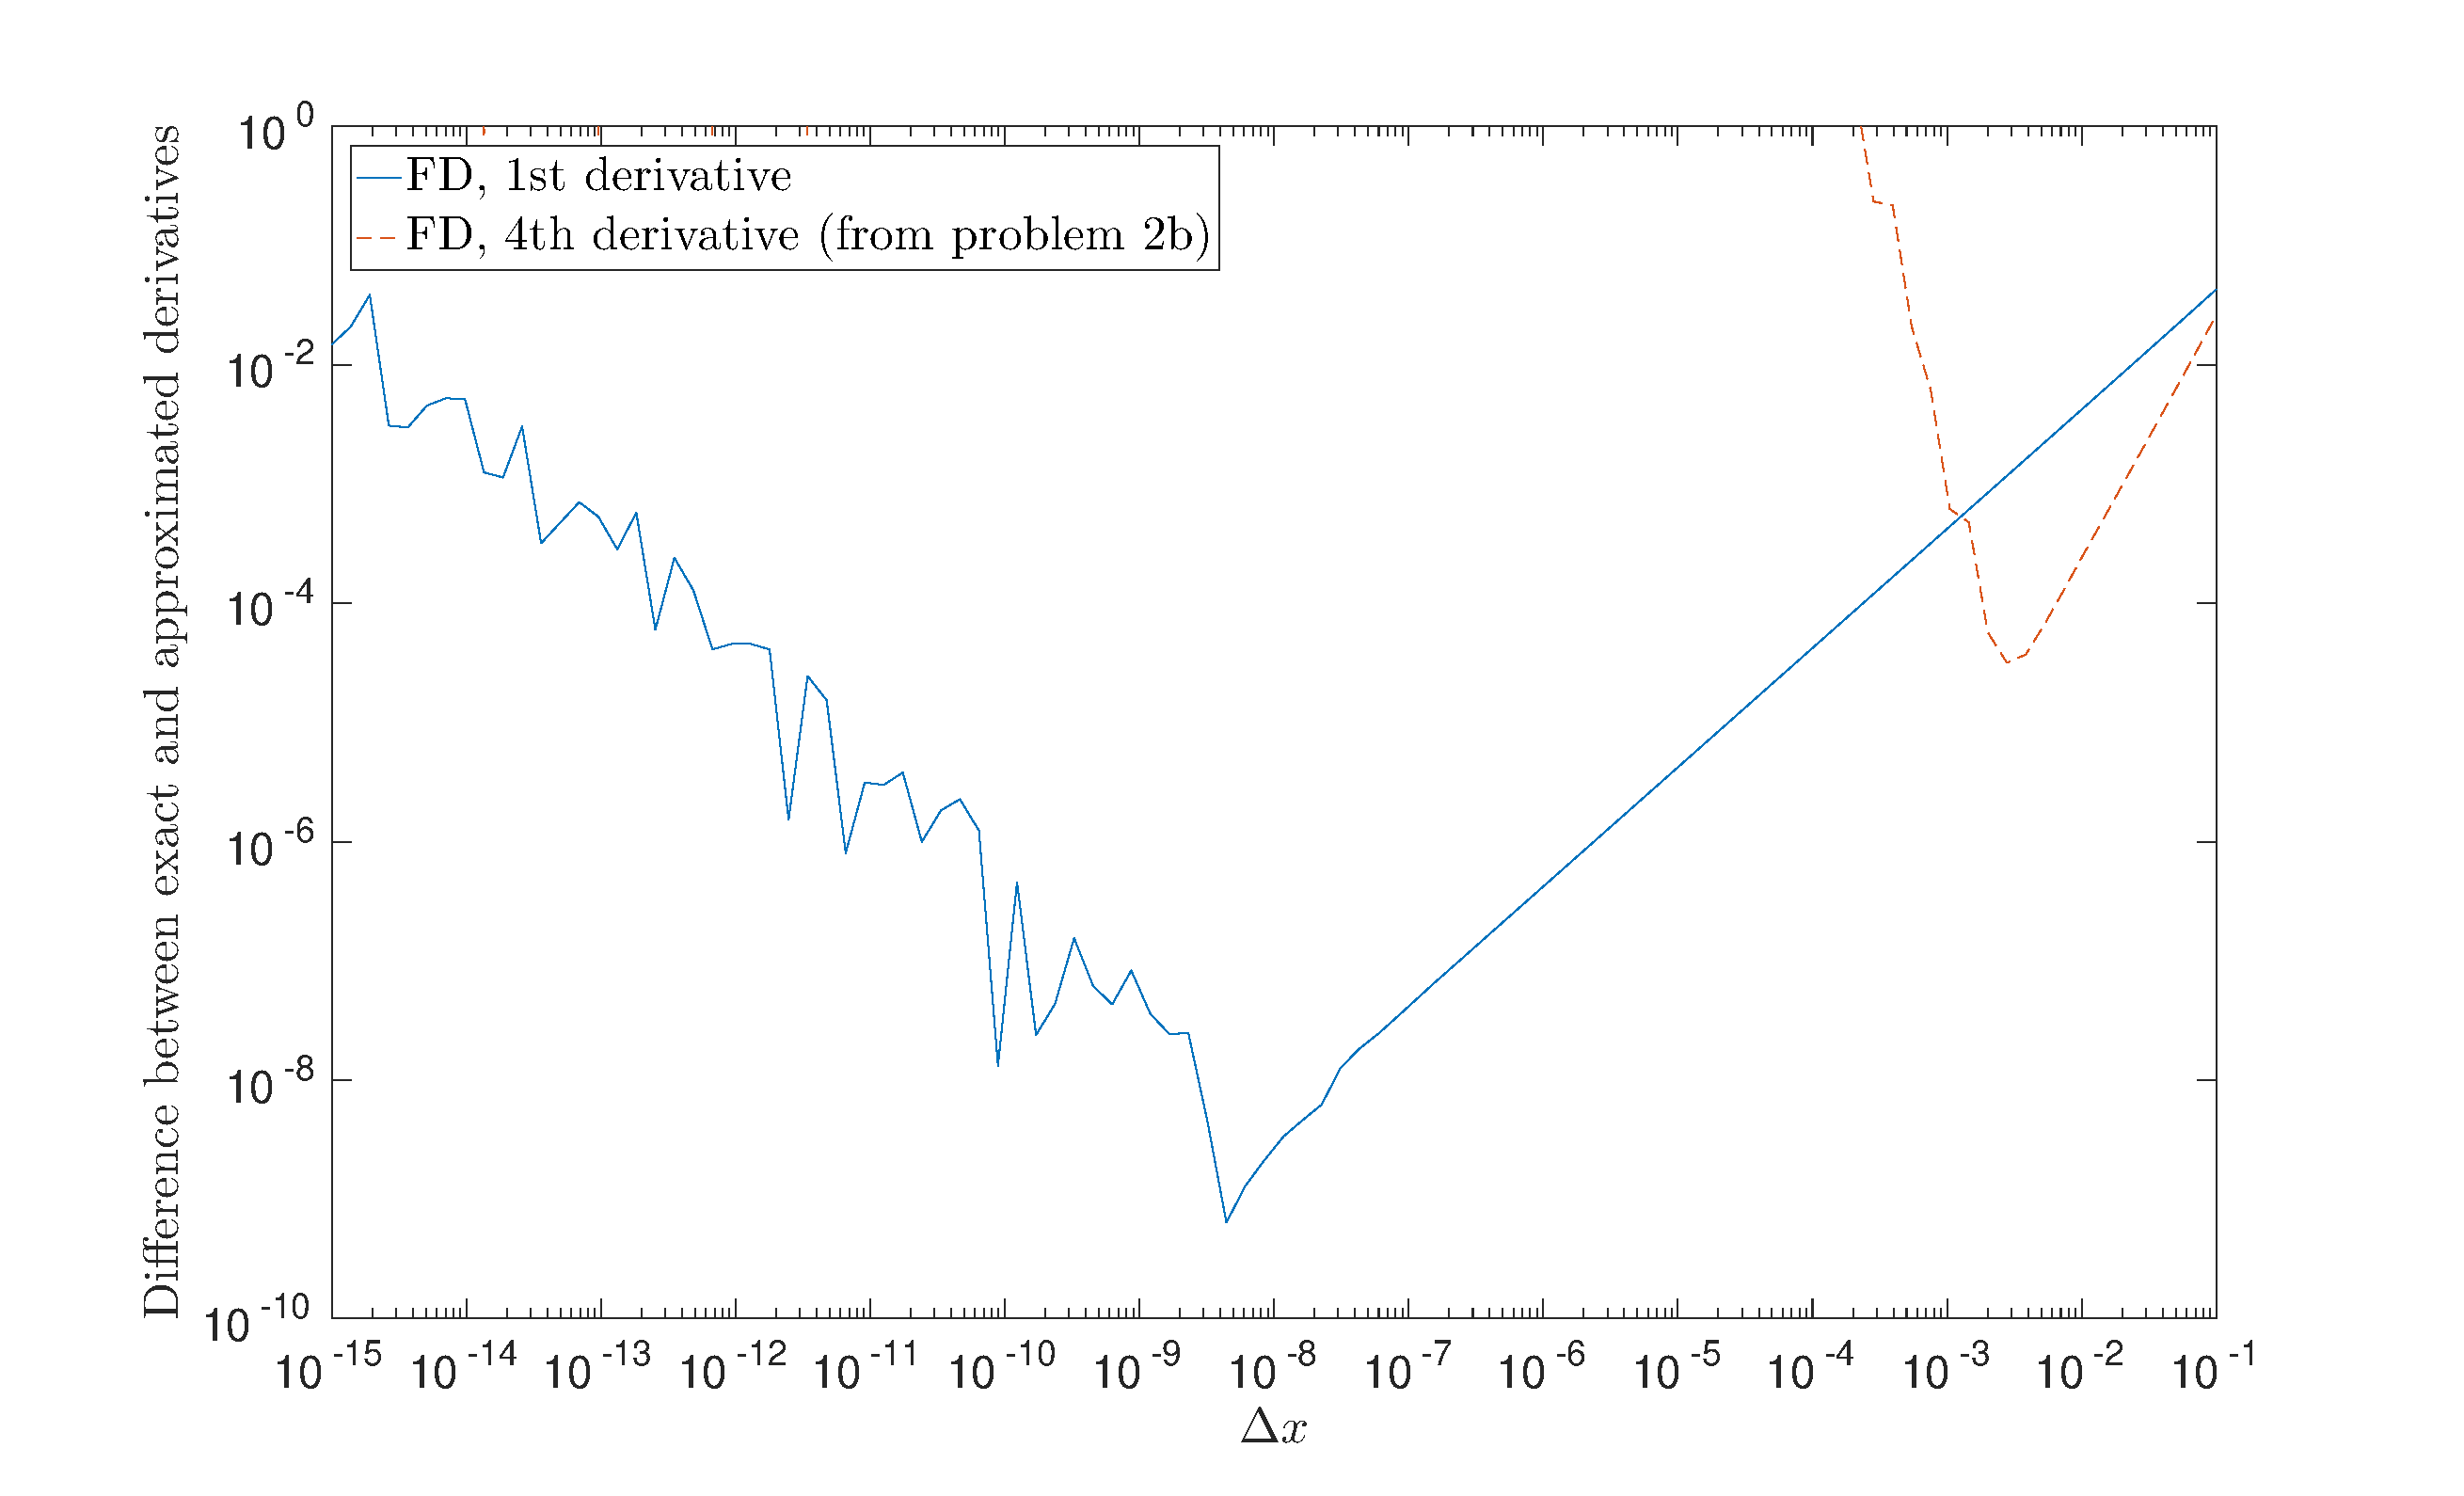
\includegraphics[width=1.2\textwidth]{3_FD.eps}}
\caption{Plot of the absolute error between approximate and ``exact''
  derivatives of $\sin(x)$ at $x=1$ as a function of the $x$-step,
  $\Dx$, used for the approximation. The asymptotic behaviors are
  also shown.}
\label{fig:3_error}
\end{figure}

In general the $d$th derivative can be approximated as
\begin{equation}\label{eq:3_du/dx}
u_{dx}=\frac{\delta^d[u, \Dx]}{\Dx^d}+\order{\Dx^E},
\end{equation}
where $\delta^d[u, x]$ is some linear combination of $u(x+i\Dx)$ for a
given set of $i$'s. Assuming $u_{dx}$ is finite we see that
\begin{equation}
\delta^d[u, \Dx]=\order{\Dx^d},
\end{equation}
meaning that the numerator in \eqref{eq:3_du/dx} will become
arbitrarily small as $\Dx\to0$. This is due to the fact that the
linear combination will be a combination of additions and subtractions
of numbers that all tends to the same value. One of the easiest
examples of this is the first FD:
\begin{equation}
u_x=\frac{u(x+\Dx)-u(x)}{\Dx}+\order{\Dx};
\end{equation}
here $u(x+\Dx)\to u(x)$ as $\Dx\to0$ so the difference in the
numerator eventually becomes too small for the floating point number
precision. 

This is true in theory with prefect real numbers. In a computer,
however, we have to do with a finite precision. This means that the
numerical scheme $\hat\delta^d$ will have some rounding error:
\begin{equation}
\hat\delta^d[u, \Dx]=\delta^d[u, \Dx]+\epsilon(\Dx),
\end{equation}
where $|\epsilon(\Dx)|\ge\epsilon_0>0$. In other words
\begin{equation}
\hat\delta^d[u, \Dx]=\epsilon(\Dx)+\order{\Dx^d}\not\to0
\quad\text{as } \Dx\to0.
\end{equation}
Any modern computer should however have a very small rounding error;
so for $\Dx$ sufficiently large, the rounding error should be negligible
compared to the discretization error.
This means that the asymptotic\footnotemark{} behavior of the errors
between the approximation and the exact derivatives are 
\begin{equation}
\hat{e}_d(\Dx)=\abs{u_{dx}-\frac{\hat\delta^d[u, \Dx]}{\Dx^d}}
\sim\begin{cases}
c_1\,\Dx^E\qcomma& \Dx\gg\Delta_0\\
c_2\,\Dx^{-d},& \Dx\ll\Delta_0,
\end{cases}
\end{equation}
where $\Delta_0$ is some threshold value for $\Dx$ where the rounding
and discretization errors are comparable in size. 
\footnotetext{This is a bit of abusing notation since $\epsilon(\Dx)$
  does \emph{not} have a limit, but will fluctuate, as $\Dx\to0$.}

We can furthermore estimate where the smallest total error will be by
estimating the error as
\begin{equation}
\hat{e}_d(\Dx)\approx\tilde{e}_d(\Dx)=c_1\Dx^E + c_2\Dx^{-d}.
\end{equation}
The minimum of $\tilde{e}_d$ will be when
\begin{equation}\label{eq:3_de/dDx}
\dv{\tilde{e}_d}{(\Dx)}=Ec_1\Dx^{E-1}-dc_2\Dx^{-d-1}=0
\end{equation}
which is when
\begin{equation}\label{eq:3_Dxmin}
\Dx_\text{min}=\qty(\frac{dc_2}{Ec_1})^{1/(E+d)}.
\end{equation}
If we're only looking for an order of magnitude estimate
\eqref{eq:3_de/dDx} can be simplified by neglecting the factors $E$
and $d$; this is the same as saying that the two types of errors are
roughly equal in size at the minimum.

\subsection{FD first derivative}
For the FD first derivative we have $d=1$ and $E=1$.
From \figref{fig:3_error}, we find the asymptotic behavior
\begin{equation}
\hat{e}_1(\Dx)=
\sim\begin{cases}
0.4\,\Dx \qcomma& \Dx\gg 10^{-8}\\
3\times10^{-17}\,\Dx^{-1},& \Dx\ll 10^{-8}.
\end{cases}
\end{equation}
Now, \eqref{eq:3_Dxmin} tells us that the minimum value should be at 
\begin{equation}
\Dx_\text{min}=\qty(\frac{1\times(3\times10^{-17})}{1\times0.4})^{1/2}
=8.7\times10^{-9}\approx 10^{-8},
\end{equation}
which agrees up to the order of magnitude with what we can see in
\figref{fig:3_error}. 


\subsection{FD fourth derivative (from 2b)}
In this case we have $d=4$ and $E=4$, and \figref{fig:3_error} gives
\begin{equation}
\hat{e}_4(\Dx)=
\sim\begin{cases}
2.5\,\Dx^2 \qcomma& \Dx\gg 10^{-8}\\
3\times10^{-15}\,\Dx^{-1},& \Dx\ll 10^{-8},
\end{cases}
\end{equation}
and 
\begin{equation}
\Dx_\text{min}=\qty(\frac{4\times(3\times10^{-15})}{1\times2.5})^{1/6}
=4.1\times10^{-3}\approx 10^{-2},
\end{equation}
which again agrees up to the order of magnitude with the result in
\figref{fig:3_error}.

\subsection*{End notes}
There are three more points I would like to address in this problem.

The first one is that $c_2$, which is roughly the rounding errors,
differs between the two derivatives. At a first glace they should be
the same, since the same machine/program should have roughly the same
rounding errors. But for the fourth derivative, $\delta_4$ involve
many more terms than in the first FD. This means that, depending on
how the additions and subtractions are carried out, there are more
instances where rounding errors are introduced. The difference, of 2
orders of magnitude, is still somewhat remarkable though. 

The second point is that it's safer to use a $\Dx_\text{min}$ rounded
\emph{up}. In this case the outcome was such that the (logarithmic)
rounding already was upwards. But it's always better to be in a
regime where you know the errors, i.e. when we don't have to worry
about rounding errors (of which we don't know the exact size).

There is ofcourse rounding errors occuring in the subtraction between
the ``exact'' and approximated derivative. Those rounding errors are
however not significant. That is because the rounding errors in the
approximation of the derivative aer divided by $\Dx\ll1$.

\subsection*{Code printout}
The calculations, done in MATLAB, for this problem is shown below; non
of the graphics code were included here.
\lstinputlisting[firstline=55, lastline=69]{code/a1.m}




\section{Numerical solution of the heat equation}
In this problem we will implement the forward time, center space
numerical scheme for the heat equation ($u_t=\sigma u_{xx}$). The scheme looks like
\begin{equation}\label{eq:4_start}
U_j^{n+1}=rU_{j+1}^n+(1-2r)U_j^n+rU_{j-1}^n,
\end{equation}
where $r=\sigma\Delta{t}/\Dx^2\le1/2$. The domain is $-1\le x\le1$ and
$t\ge0$, with IC $u(x,0)=\sin(\pi x)$ and BC $u(-1,t)=u(1,t)=0$.

We begin by noting that the equation \eqref{eq:4_start} is a linear
transformation:
\begin{equation}
\vb*{U}^{n+1}=\mathsf{A}\vb*{U}^n.
\end{equation}
It is easy to realize that $\mathsf{A}$ must be a matrix with
$(1-2r)$ on its diagonal and $r$ on the first upper and lower
off-diagonals. But to implement the BC, we need the end element to be
0, which can be realized by setting the ends of the off-diagonals to 0
at the top and bottom row of $\mathsf{A}$:
\begin{equation}
\mathsf{A}=
\begin{bmatrix}
(1-2r)&0&0&0&0&\ldots&0\\
r&(1-2r)&r&0&0&\ldots&0\\
0&r&(1-2r)&r&0&\ldots&0\\
\vdots& & & \cdots& &&\vdots\\
0&\ldots&0 &0&r&(1-2r)&r\\
0&\ldots&0 &0&0& 0&(1-2r).
\end{bmatrix}
\end{equation}
Afterwards it's just a matter of looping trough all the time steps. 
\\[11pt]
This method is implemented in the piece of MATLAB code below:
\vspace{-14pt}
\begin{lstlisting}
sigma=1;
dX=0.01; %mesh size
r=.4;
X=-1:dX:1; %the mesh
N=length(X);
T=.1;%end time
dt=(r*dX^2/sigma);%dt is chosen based on what r value we want
n=floor(T/dt);

u0=sin(pi*X).'; %IC

% the linear transformation that gives us the next time step:
A=(1-2*r)*eye(N)...%the diagonal
  ...% vvv--- the off-diagonal elements ---vvv
   +[zeros(N-1,2),[zeros(1,N-2); r*eye(N-2)];zeros(1,N)]...
   +[zeros(1,N);[r*eye(N-2);zeros(1,N-2)],zeros(N-1,2)];

U=[u0,zeros(N,n-1)];%init
for i=2:n %Solving for all t
    U(:,i)=A*U(:,i-1);
end
\end{lstlisting}


\subsection{Simple numerical solution}
\begin{figure}\centering
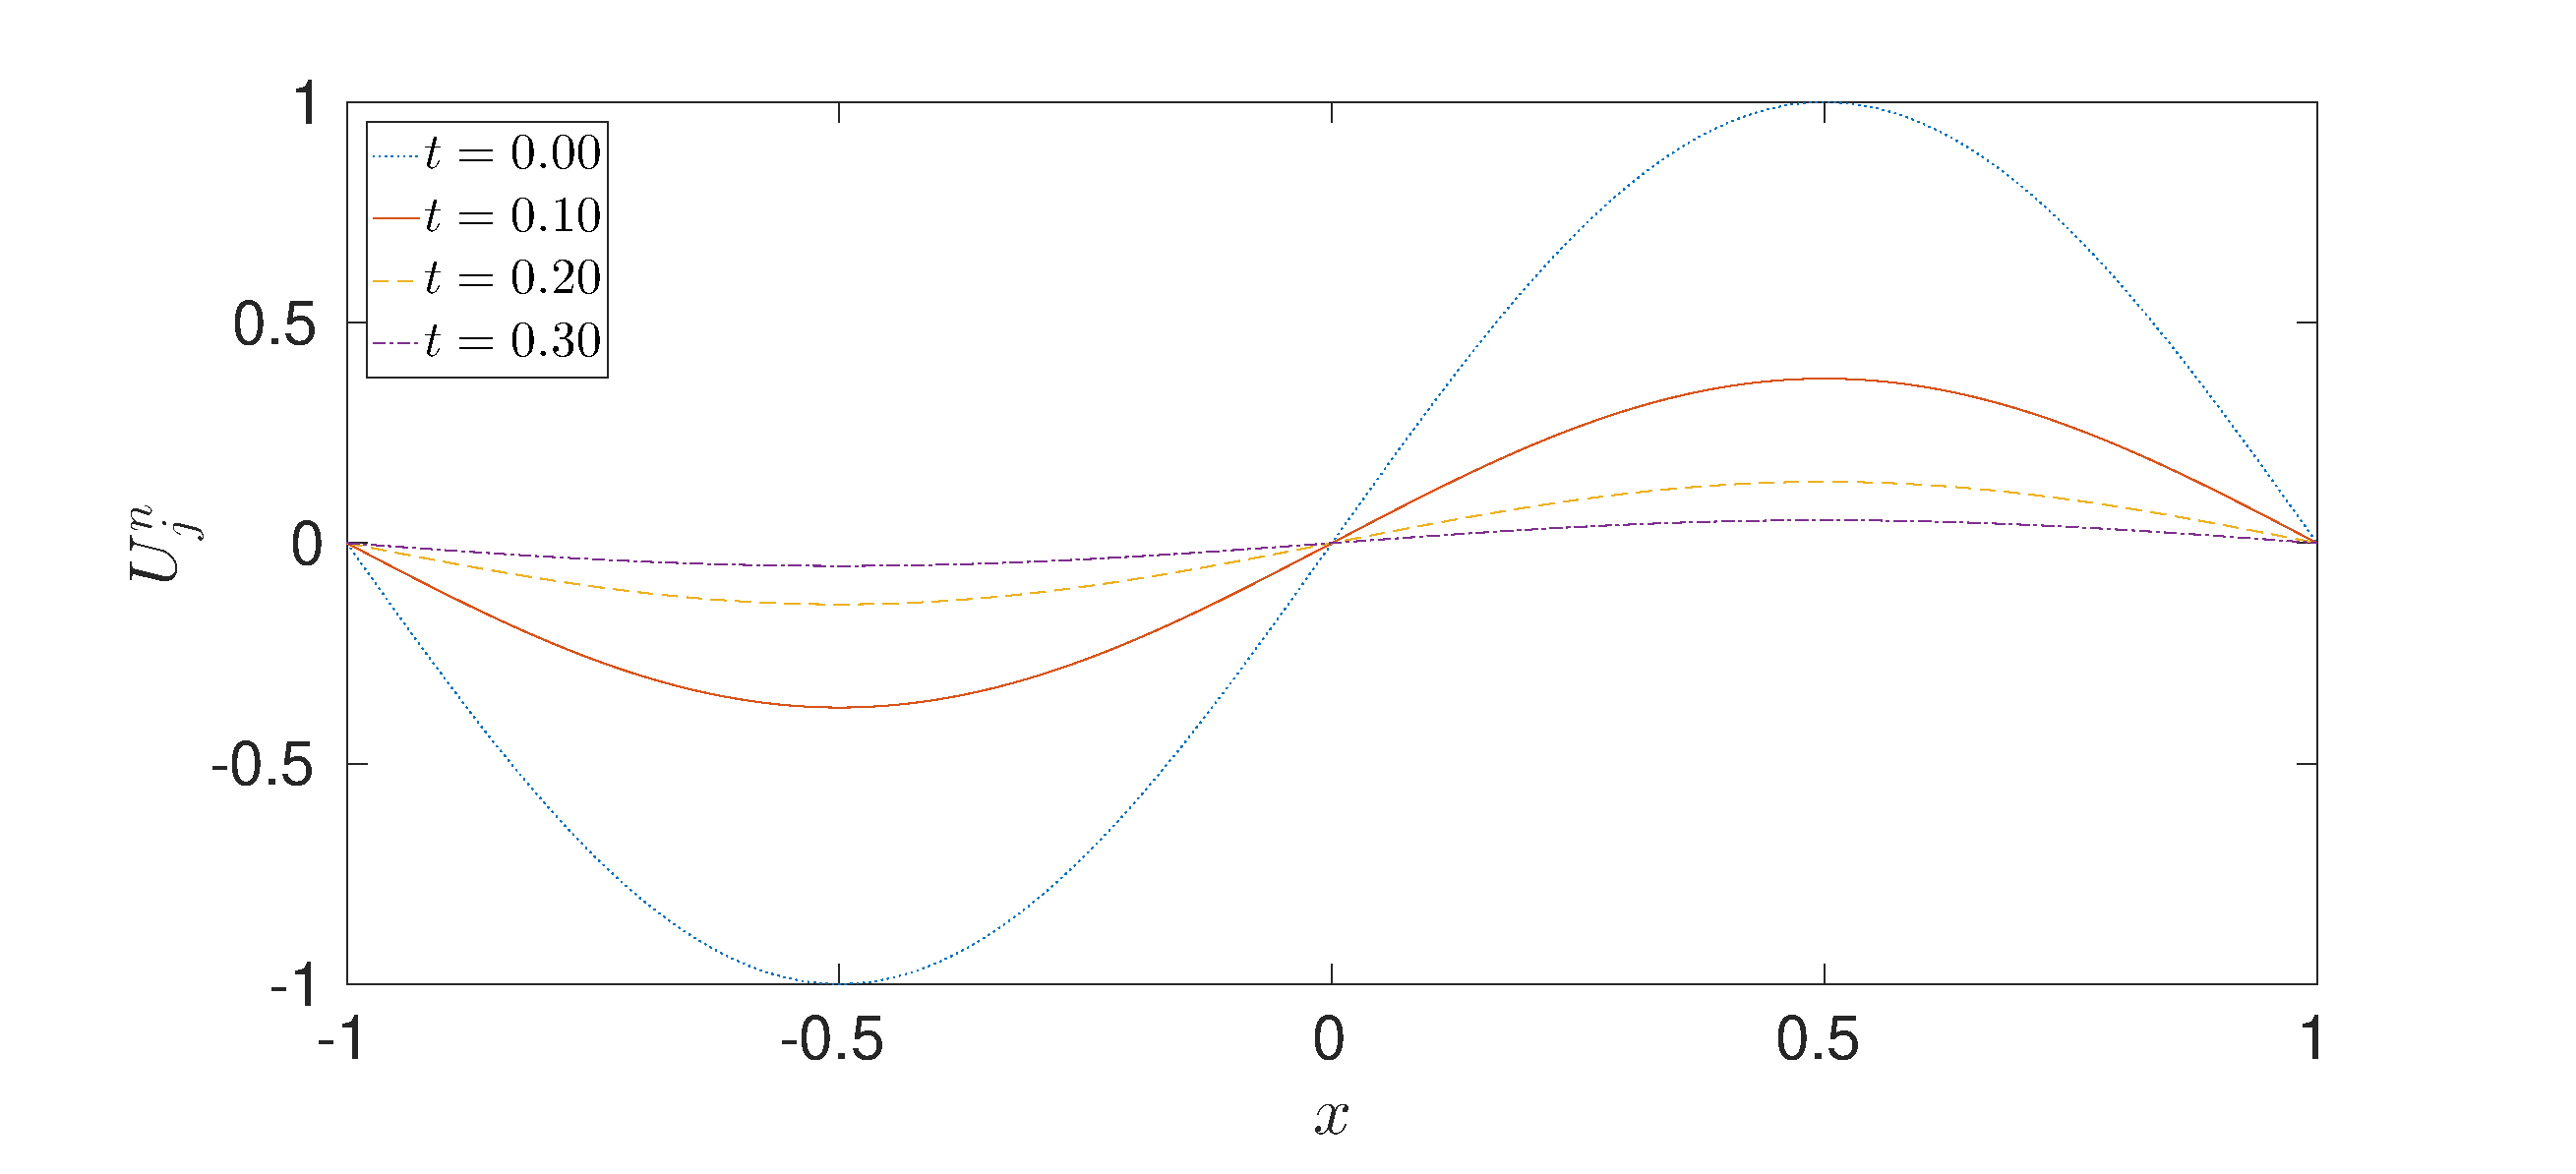
\includegraphics[width=1\textwidth]{4a.eps}
\caption{Numerical solution to the heat equation at different times,
  with $\sigma=1$, $\Dx=0.01$ and $r=\sigma\Delta{t}/\Dx^2=0.4$. }
\label{fig:4a}
\end{figure}

\figref{fig:4a} shows solutions, using the code provided above, at some
different times. We see that the general behavior of the solution is
that the solutions decay over time. In this specific case, we only
have one frequency so we can not see any difference in decay rate
between frequencies --- as we would have expected otherwise. In the
end the solution will tend towards no fluctuations, that is $U_j^n\to
0$ for all $j$ as $n\to\infty$


\subsection{Varying $\sigma$}
\begin{figure}\centering
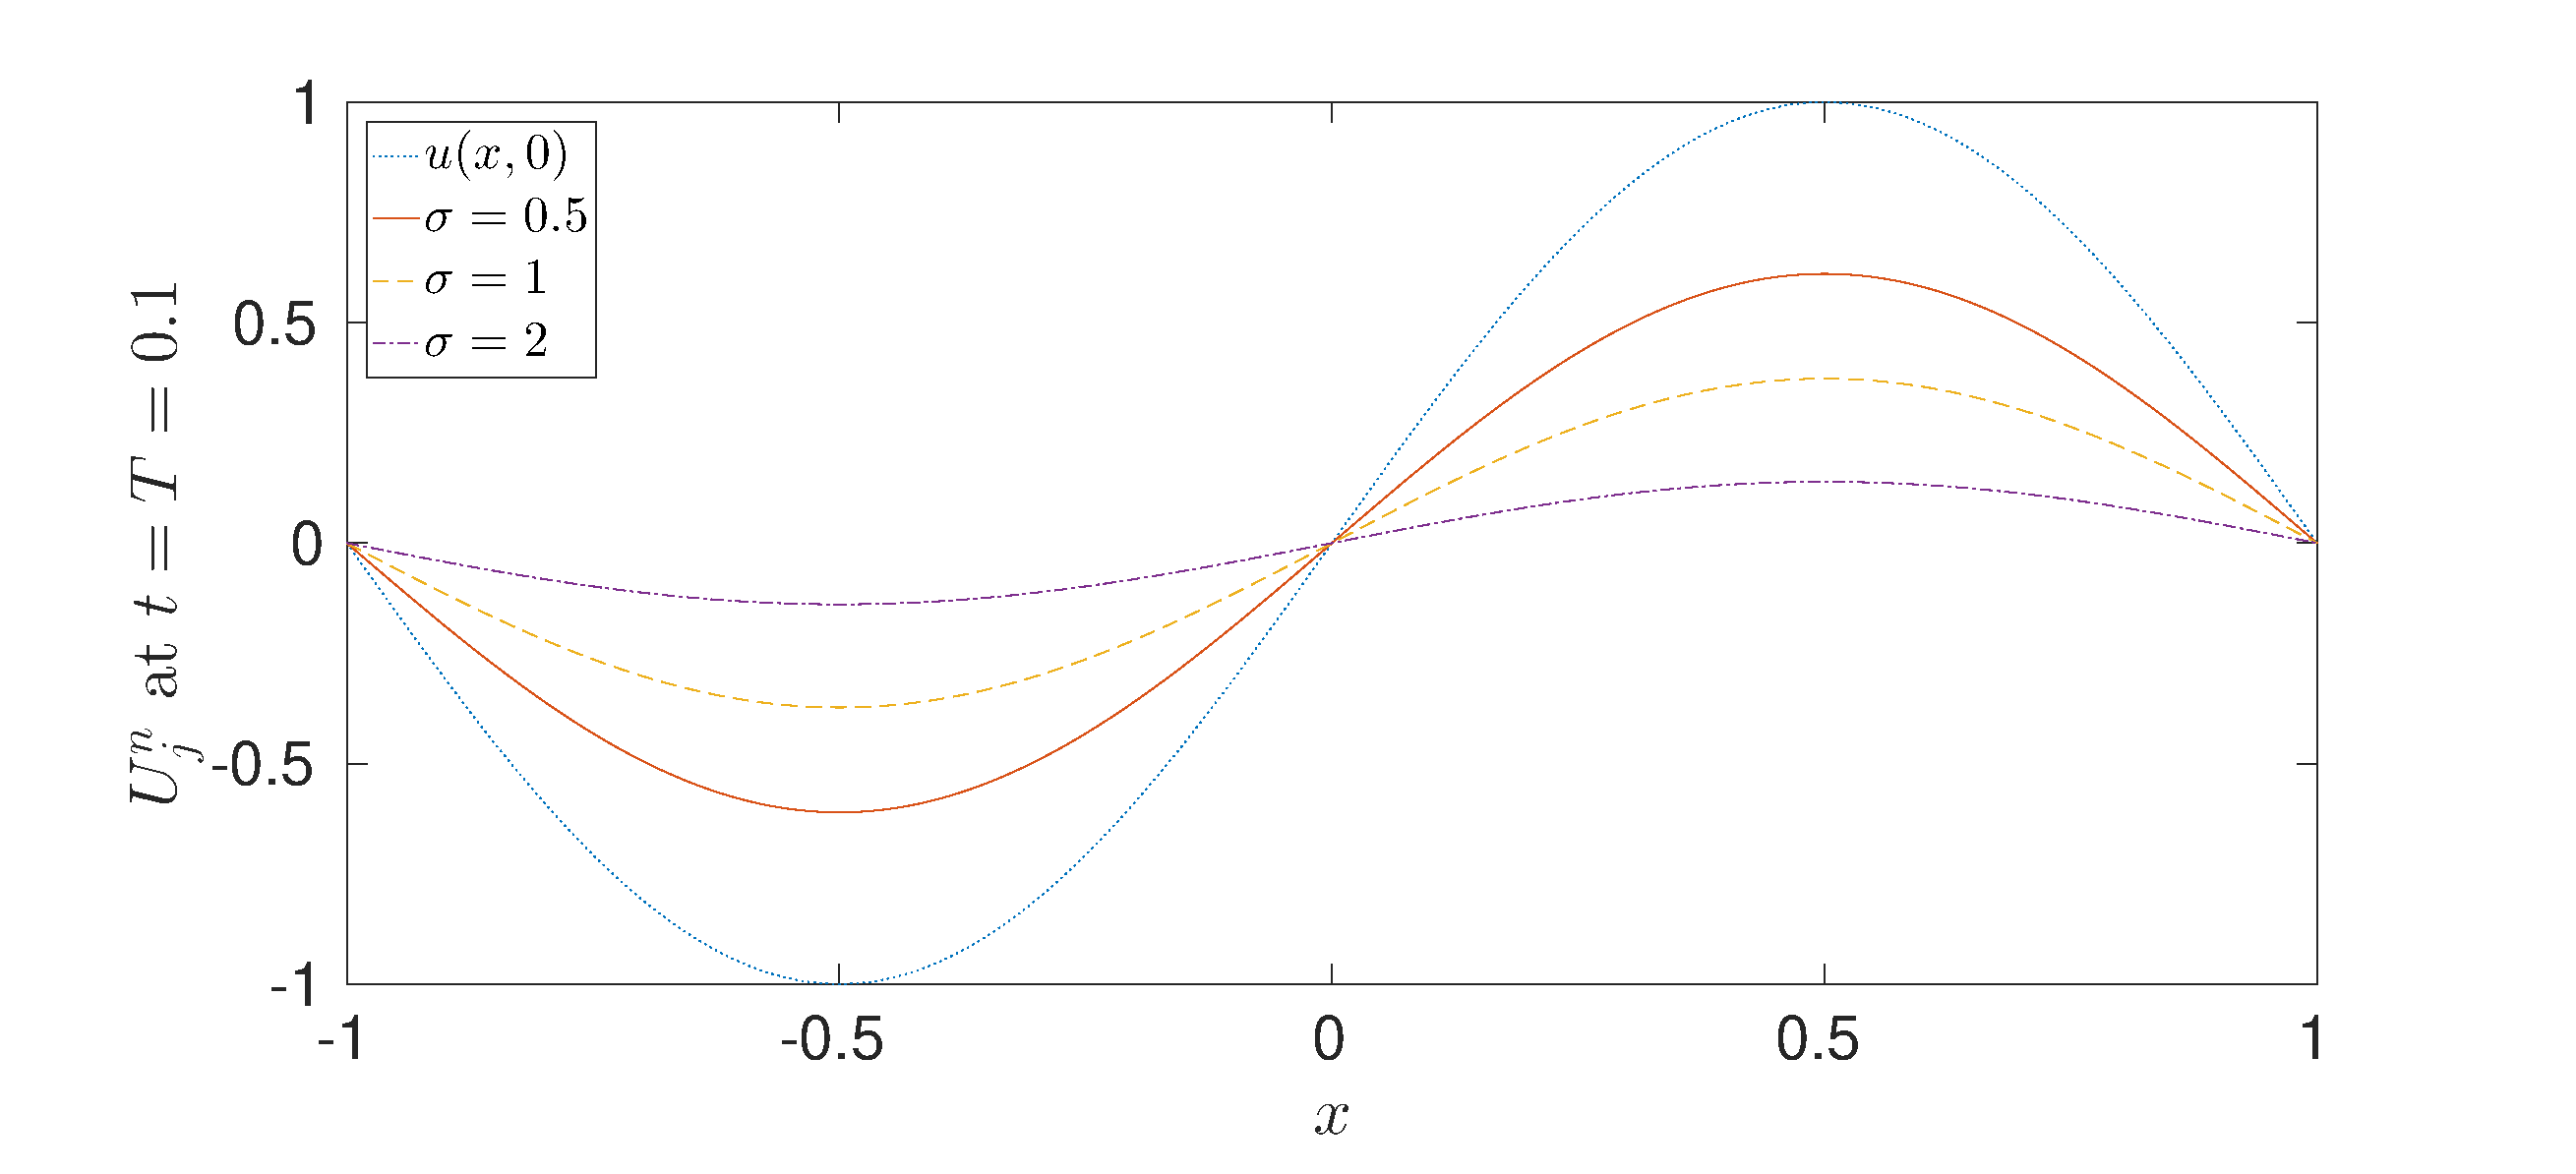
\includegraphics[width=1\textwidth]{4b.eps}
\caption{Numerical solution to the heat equation with different
  diffusion coefficients,
  at $t=0.1$, $\Dx=0.01$ and $r=\sigma\Delta{t}/\Dx^2=0.4$. }
\label{fig:4b}
\end{figure}

The result of the numerical scheme is shown in \figref{fig:4b}.
We see here that a greater diffusion coefficient makes for stronger
decay of the solution. That is also what we would have expected from
the exact solution.

\subsection{Varying $\Dx$}
\begin{figure}\centering
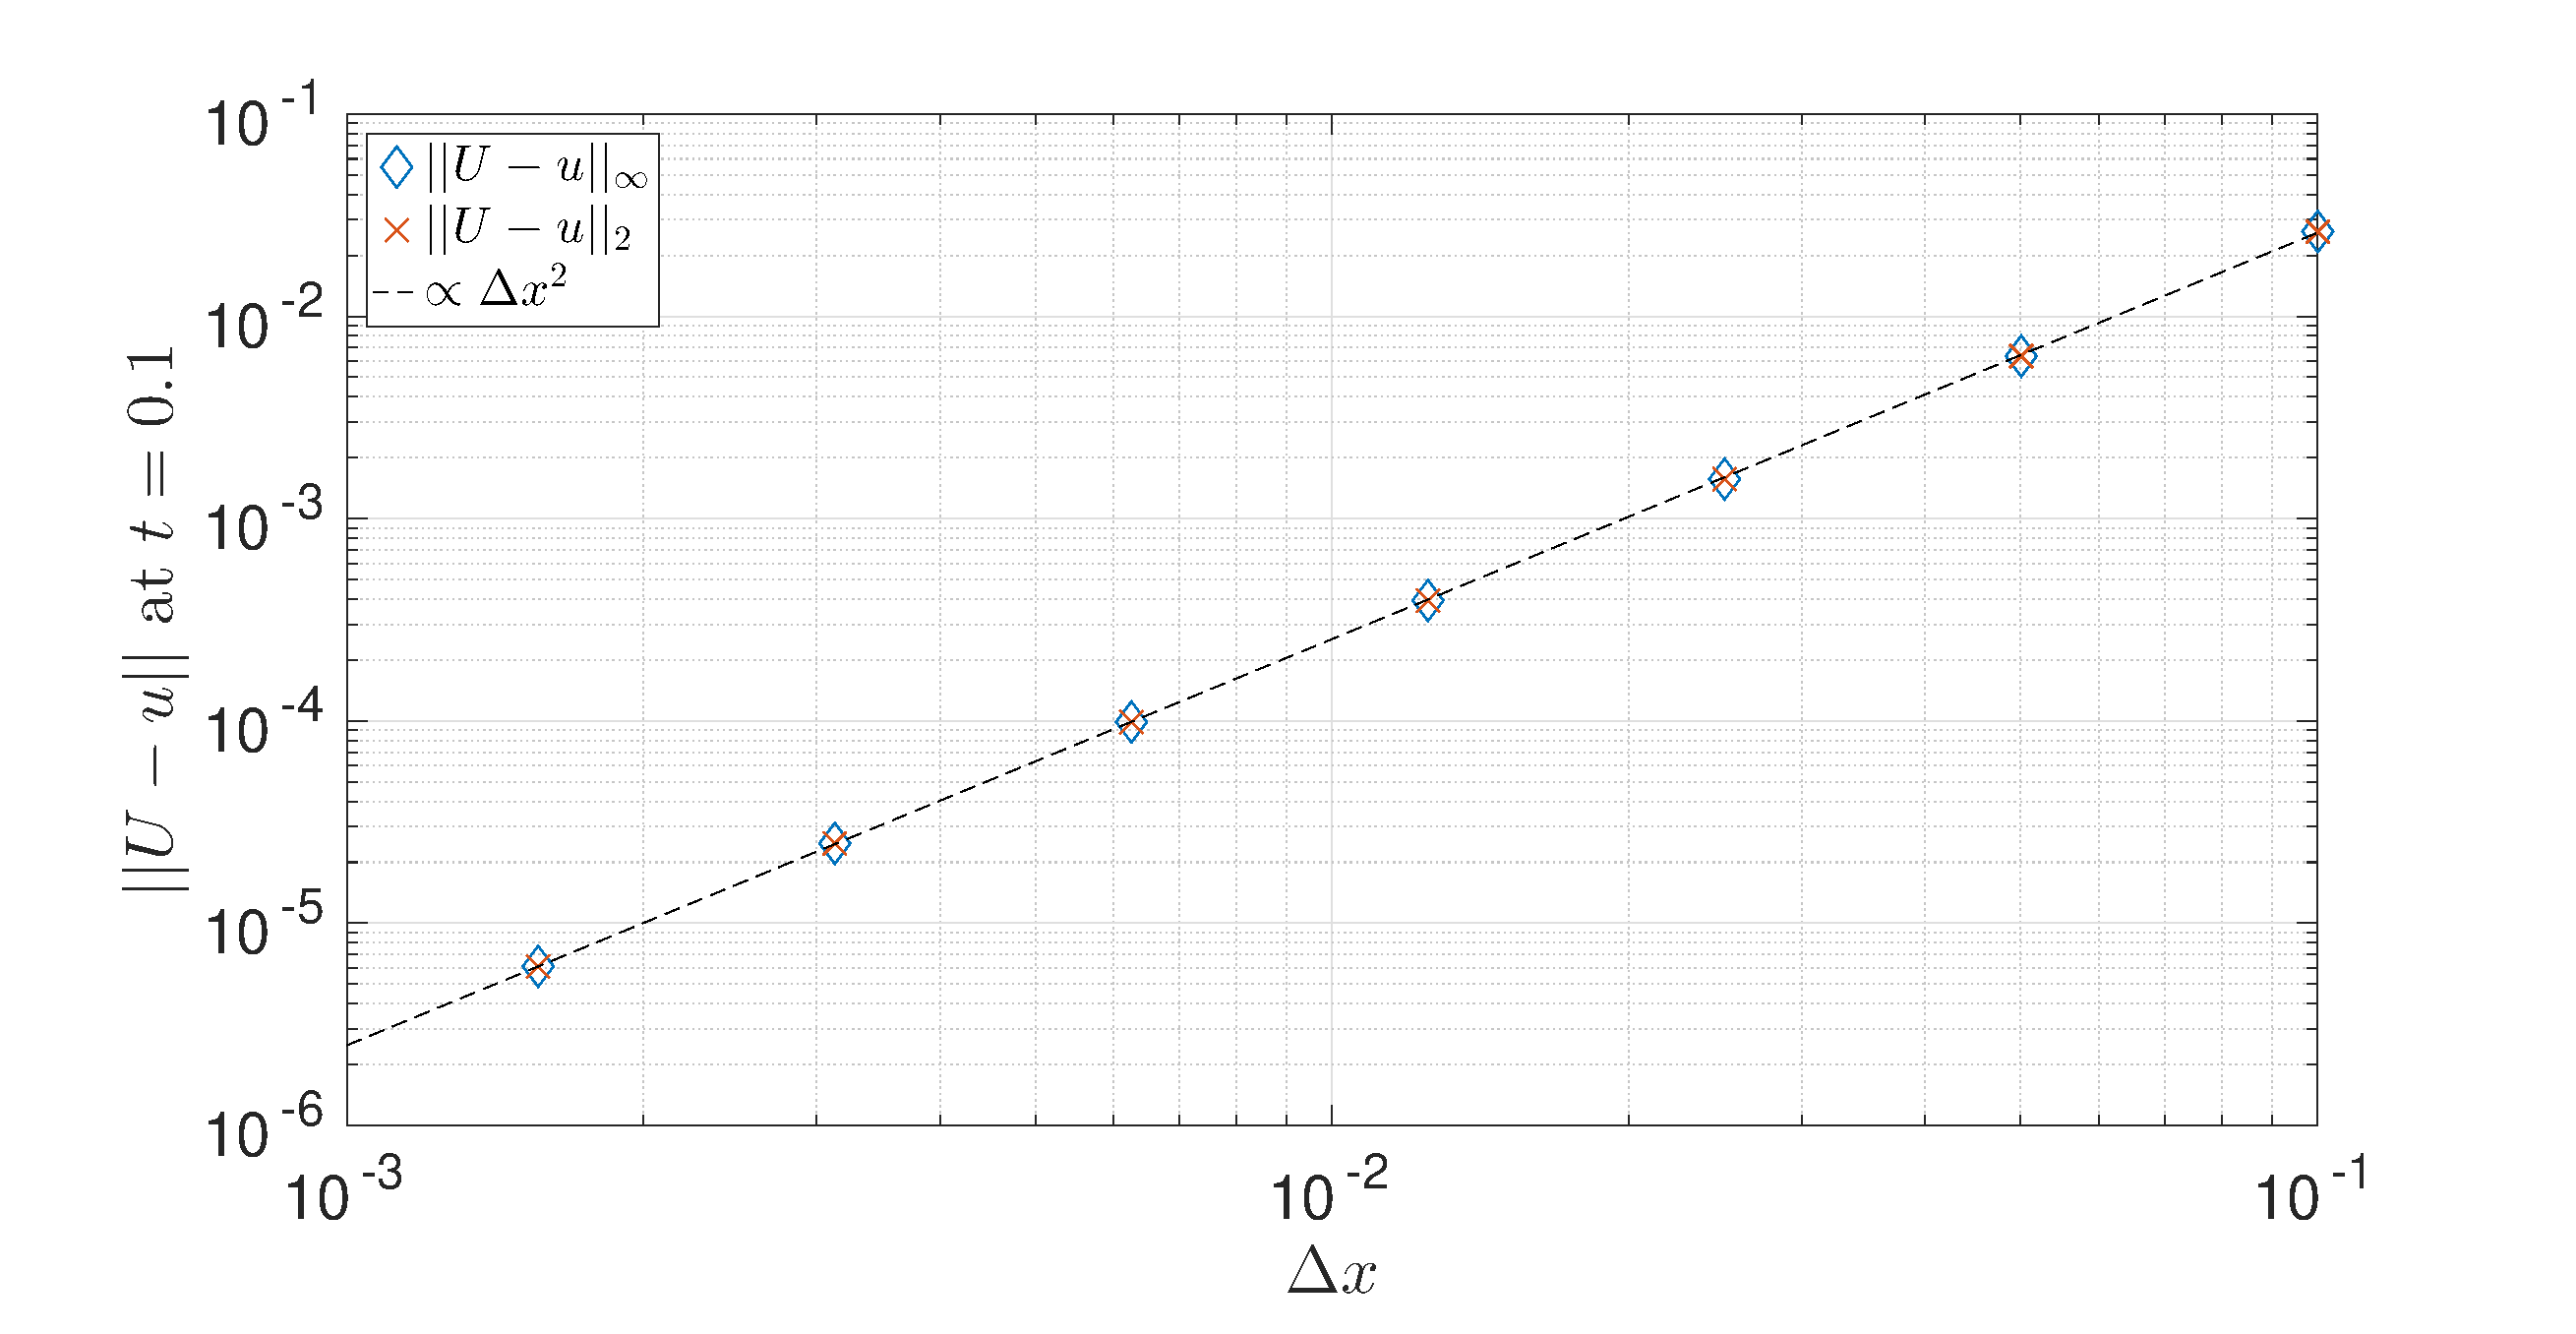
\includegraphics[width=1\textwidth]{4c.eps}
\caption{The error between the numerical and exact solution to the
  heat equation with different mesh sizes, at $t=0.1$, $\sigma=1$ and
  $r=0.4$ (fixed for all $\Dx$). }
\label{fig:4c}
\end{figure}

Here we're going to study how the the error between the numerical
and the exact solution is affected by the mesh size $\Dx$. To do this
we implement two different norms. The first norm is just the regular
max-norm, and the second one is a scaled 2-norm:
\begin{equation}
||U-u||_2=\sqrt{\Dx\sum_{j=1}^J(U_j-u_j)^2}.
\end{equation}

The result is shown in the table below and in \figref{fig:4c}. We see
that the two different norms are exactly the same (to the 4th decimal
place), which was very unexpected. 
%\begin{table}
\begin{center}
\begin{tabular}{|l|c|c|c|c|c|c|c|}\hline
$||U-u||_\infty\times10^3$&26.3436&6.3680&1.5789&0.3939&0.0984&0.0246&0.0062\\
\hline
$||U-u||_2\times10^3$&26.3436&6.3680&1.5789&0.3939&0.0984&0.0246&0.0062\\
\hline
\end{tabular}
\end{center}
% \end{table}

From the log-plot in \figref{fig:4c}, we see that the rate of
convergence is quadratic.

\end{document}




%  LocalWords:  MFT MF Advection PDE's AMATH IC discretization MATLAB
